\documentclass{dialogue}

%\usepackage{bookta}sb

\begin{document}
	
	\begin{otherlanguage}{english}
		\begin{center}
			{\Large\bfseries{Joint task learning for relation extraction and named entity recognition}}
			% Relation extraction as sequence labelling and the failed case of joint task learning
			% Joint task learning for relation extraction and named entity recognition
			% JORN: Joint Relation extraction and named entity recognition
			% Everything is a Sequence: Relation Extraction and Named Entity Recognition as Sequence Labelling
			% ReNErSANs: Relation Extraction and Named Entity Recognition as Sequence Annotation
			
			\medskip
			
			%Adis Davletov (\texttt{davletov-aa@ranepa.ru}), Denis Gordeev (\texttt{gordeev-di@ranepa.ru}), Alexey Rey (\texttt{rey-ai@ranepa.ru}) Nikolay Arefyev (\texttt{nick.arefyev@gmail.com})
			Authors
			
			\medskip
			
			%RANEPA, Moscow, Russia
			Institution
		\end{center}
		
		In this work we present our system for RuREBus challenge held together with Dialog 2020 conference. The task consisted of 3 subtasks: named entity recognition, relation extraction with provided named entity tags and end-to-end relation extraction. Our system took the first and the second place in the first and the second subtasks respectively. For the second subtask we submitted our solution only in the post-evaluation phase, however, it was among top 2 best performing systems. The systems for all tasks are based on Transformer models. Relation extraction was solved as a sequence labelling problem. We also used joint task named entity and relation extraction learning \footnote{https://github.com/AdisDavletov/DeftEval2020/tree/dev}.
		
		\textbf{Key words:} Relation Extraction, Named Entity Recognition, Transformer, BERT
	\end{otherlanguage}
	
	\bigskip
	
	\begin{otherlanguage}{russian}
		\begin{center}
			{\Large\bfseries{Совместное обучение моделей для извлечения отношений и именованных сущностей}}
			%Совместное обучение моделей для извлечения отношений и именованных сущностей
			
			\medskip
			
			%Давлетов А. А. (\texttt{davletov-aa@ranepa.ru}), Гордеев Д. И. (\texttt{gordeev-di@ranepa.ru}), \\Рей А. И. (\texttt{rey-ai@ranepa.ru}), Арефьев Н. В. (\texttt{nick.arefyev@gmail.com})
			Авторы
			
			\medskip
			
			%РАНХиГС, Москва, Россия
			Организация
		\end{center}
		
		В данной работе мы представляем нашу систему для соревнования RuREBus, проводящегося совместно с конференцией Dialog 2020. Задача состояла из 3 дорожек: распознавание именованных сущностей, классификация отношений между заранее аннотированными именованными сущностями и извлечение отношений из неаннотированного текста. Наша система заняла первое место на первой дорожке и второе место на третьей. Для второй задачи мы не успели своевременно представить решение, но оно бы оказалось в числе лучших систем. Системы для всех задач основаны на моделях Transformer. Извлечение отношений мы рассматривали как задачу разметки последовательностей. Также мы использовали совместное обучение для задач распознавания именованных сущностей и извлечения отношений.
		
		% Relation extraction was solved as a sequence labelling problem. We also used joint task named entity and relation extraction learning.
		\medskip
		
		\textbf{Ключевые слова:} извлечение отношений, распознавание именованных сущностей, Transformer, BERT
	\end{otherlanguage}
	
	\selectlanguage{english}
	
	\section{Introduction}
	This work is devoted to RuREBus challenge held together with the conference Dialog 2020. RuREBus competition was devoted to the problem of relation extraction and named entity recognition (NER) in a specialized business domain. The competition consisted of three subtasks: named entity recognition, relation extraction with provided named entity labels and end-to-end relation extraction. Our first subtask solution was a BERT-based \cite{bert} sequence labelling model. For the second one we applied joint named entity and relation extraction learning. We went with a similar approach for the third subtask. However, due to having no labelled named entities, they were inferred using the model trained for the first subtask.
	
	Our NER model with the 0.561 F1-score at the test dataset took the first place in the competition. Our second subtask model took the second place with the F1-score equal to 0.394.
	
	Our work shows that the sequence labelling approach is viable for relation extraction. It also demonstrates that correct named entity labels are vital for relation extraction due to the difference in scores between the second and the third subtask models.
	
	\section{Related work}
	There are many ways to extract information from text. This task is often solved by extracting named entities and classifying relations between them. One of the most popular datasets for this task is TACRED \cite{tacred} where semantic relations are understood as relations between two pairs of entities.
	
	Nowadays, state-of-the-art results for this dataset are achieved with Transformer-based models \cite{attention}. The most advanced models (according to paperswithcode\footnote{https://paperswithcode.com/sota/relation-extraction-on-tacred}) use extra training data or additional knowledge bases. For example, in \cite{BaldiniSoares2019} the authors use Wikipedia data. However, such data is useless for domain-specific relations.
	
	Among the systems that do not use encyclopedias or other labeled data, the best results were achieved by Joshi et al. \cite{spanbert}. They pre-trained a BERT-like system, but instead of predicting individual masked tokens they trained the model to infer contiguous random spans. The model was also trained to predict each token in the masked span using output representations of only span boundary tokens. This significantly improved results of their model in comparison with the vanilla BERT. As in both described works we also incorporated information about named entity spans.
	
	However, it is difficult to compare results for relation extraction systems for languages besides English because such annotated datasets are scarce for most languages including Russian. Some researchers have tried to solve this problem using unsupervised language-agnostic approaches and relying on knowledge databases such as Wikidata and various online encyclopedias such as Wikipedia \cite{Heist2017}. Models trained this way tend to be not specialized because the original database does not contain relations from the required domain. The results are good only for the most popular relation types such as geographical or professional ones, which frequently appear in Wikipedia.
	
	\section{Shared task overview}
	The organizers of the competition have provided approximately 300 annotated texts in total. All texts were provided by the Ministry of Economic Development of the Russian Federation. The corpus consists of various regional and strategic plan reports. There are in total 8 named entity classes and 11 semantic relation classes (see Tables \ref{tab:ner} and \ref{tab:rel}). The organizers have also provided a large unannotated dataset for language model fine-tuning. However, we did not use it. A named entity can consist of several words. All entities and relations do not span across sentences. There may be many-to-many, many-to-one and other types of relations (see Fig. \ref{fig:brat}).
	
	\begin{figure}[thb]
		\centering
		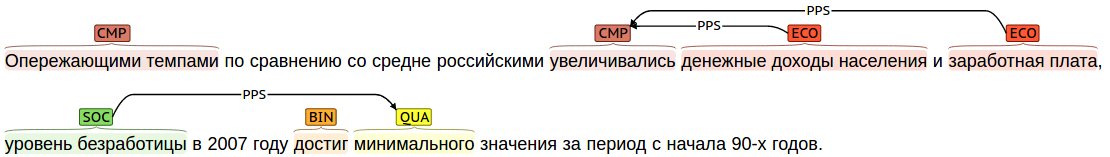
\includegraphics[scale=0.4]{pics/brat}
		\caption{RuREBus annotation example.}
		\label{fig:brat}
	\end{figure}
	
	
	Named entity groups could contain rather broad types of entities, for example "SOC" entities contained social groups as well as various social attributes - phrases like 'blue collar workers' and 'housing accessibility' corresponded to this group.
	
	\begin{table}[bth]
		\centering
		\small
		\begin{tabular}{p{0.7cm}|p{4cm}|p{10cm}}
			\hline
			Type & Description & Examples\\ \hline
			MET & Some quantitative metric & доля сельского населения (rural population ratio); положение в округе (ranking in the neighbourhood)\\ \hline
			ECO & An economy entity or facility & обрабатывающим сектором промышленности (processing industry); экономического кризиса (economic crisis) \\ \hline
			BIN & A binary attribute & входит в состав (is part of)\\ \hline
			CMP & Comparative attribute & рост (growth); увеличился (increased); в наибольшей степени (to the greatest extent)\\ \hline
			QUA & Qualitative attribute & лидирующее (leading)\\ \hline
			ACT & Activity, actions, implemented policies & восстановление экономики региона {region economy reconstruction}\\ \hline
			INST & Institutions and organizations & Алтайского края (Altai region); Сибири (Siberia)\\ \hline
			SOC & Social groups and characteristics & населения края (region population); здравоохранение (health care) \\ \hline
		\end{tabular}
		\caption{Named entity types}
		\label{tab:ner}
	\end{table}
	\begin{table}[bth]
		\centering
		\small
		\begin{tabular}{p{3.7cm}|c|p{3.8cm}}
			\hline
			Group & Type & Description\\ \hline\hline
			Current state of affairs & NNG & now negative \\ \hline
			Current state of affairs & NNT & now neutral \\ \hline
			Current state of affairs & NPS & now positive \\ \hline\hline
			
			Results & PNG & past negative\\ \hline
			Results & PNT & past neutral\\ \hline
			Results & PNS & past positive\\ \hline\hline
			
			Forecasts & FNG & future negative\\ \hline
			Forecasts & FNT & future neutral\\ \hline
			Forecasts & FNS & future positive\\ \hline\hline
			
			Goals & GOL & some abstract goals\\ \hline
			Tasks & TSK & tasks and actions performed to achieve goals\\ \hline
			
		\end{tabular}
		\caption{Semantic relation types}
		\label{tab:rel}
	\end{table}
	
	The organizers first held tracks 1 and 3 and after that track 2 was also run. We describe our solutions in the same order (first tracks 1 and 3, then track 2).
	\section{Named entity recognition and relation extraction as sequence labelling}
	The data for the competition was presented in brat format \cite{brat} where texts were given as plain text files and annotations were provided in another file with mixed labels for named entities and relations between them. Thus, we first had to separate the labels and transform the data into special formats used by our models.
	
	We used Razdel library to split plain texts into sentences and tokens \footnote{https://github.com/natasha/razdel}. It is a rule-based system that along with splitting sentences can also provide sentence and token offsets in the source text. Offset ranges provided by Razdel were used during preprocessing and postprocessing to map tags and relations to text spans which are required by the brat format (see Table \ref{tab:tokenization}).
	
	\begin{table}[bth]
		\centering
		\begin{tabular}{c|c|c|c|c}
			\hline
			\multicolumn{1}{c|}{Dataset} &
			\multicolumn{4}{c}{Number of} \\  \hline
			& Sentences& Tokens & NER tags & Original NER tags\\ \hline
			train & 10460 & 336023 & 54377 & 54388\\ \hline
			test & 20483 & 643668 & 89006 & 89879\\ \hline
		\end{tabular}
		\caption{Named entity types}
		\label{tab:tokenization}
	\end{table}
	
	\subsection{Subtask 1: Named Entity Recognition}
	The first task was to annotate named entities. First we transformed the data into format where in each example we have pairs of tokens and their corresponding tags. Sentences were separated with newlines. We randomly split the data into training and validation datasets in 0.7 to 0.3 ratio. After hyperparameter tuning we did not retrain the model using the left validation data. We used a BERT-based system \cite{bert} with PyTorch model code and pretrained weights provided by Hugging Face \cite{Wolf2019HuggingFacesTS}. Due to competition being in Russian, we used the multilingual uncased base BERT model.
	
	BERT is a Transformer based model \cite{attention}. On top of BERT outputs we added a linear layer with softmax activation function and dropout regularization. The cross entropy loss function was used to train the model. For each word token in the sentence we took a BERT embedding from its first BPE-token and fed it to the dropout layer followed by the linear layer. All non entity tokens were ignored (i.e. padding tokens and tokens describing borders between sentences and various spans).
	
	\begin{table}[t!bh]
		\centering
		\scriptsize
		\begin{tabular}{lcc}%{llllllll}

			Method & test & dev \\

			test\_xlm\_r\_tag\_0.1\_wd\_0.2\_relation\_run\_predictions & 0.497 & 0.465 \\
			test\_xlm\_r\_tag\_0.01\_relation\_run\_predictions & 0.33 & 0.294 \\
			test\_xlm\_r\_tag\_0.1\_relation\_drop\_0.2\_run\_predictions & 0.489 & 0.456 \\
			$\star$ whole\_train\_tag\_0\_xlm\_r\_run\_predictions & 0.002 & 0.003 \\
			test\_xlm\_r\_tag\_relation\_run\_predictions & 0.465 & 0.463 \\
			test\_xlm\_r\_tag\_0.1\_relation\_run\_predictions & 0.494 & 0.467 \\
			test\_xlm\_r\_tag\_0\_relation\_run\_predictions & 0.0398 & 0.0495 \\
			test\_xlm\_r\_tag\_0.05\_relation\_run\_predictions & 0.482 & 0.440 \\
			test\_tag\_0.1\_and\_relation\_run\_predictions & 0.189 & 0.172 \\
			test\_tag\_0\_and\_relation\_run\_predictions & 0.002 & 0.001 \\
			test\_xlm\_r\_tag\_0.2\_relation\_run\_predictions & 0.503 & 0.468 \\

		\end{tabular}
		\caption{Subtask 1: Results on test and development sets on multitask system. $\star$ denotes out of competition result}
		\label{table:test_results}
	\end{table}
	
	Our system with 0.561 micro F1-score on the public leaderboard outperformed solutions presented by other contestants.
	
	\subsection{Subtask 3: End-to-end Relation Extraction}
	The second and the third subtasks were relation classification. In the second subtask the organizers provided named entity tags while in the third they did not. For both tracks we used the equivalent approach.
	
	Akin to BERT-multitask learning, in this competition we wanted to experiment with simultaneous finetuning for separate tracks. RuREBus competition provided an excellent framework for this idea because we had separate tracks with different target values but the same input data. Thus, we tried a multitask architecture to jointly predict tags and relations. To do so, we consider relation extraction as a sequence labeling problem (similar to how named entity recognition is usually solved). In each example we have one marked main entity and we predict all named entity tags and all relations between the main token and all other tokens in the sentence (see Fig. \ref{fig:rel}). We put an empty relation label (‘0’) if a token does not have relation to the marked entity and the relation tag otherwise. Special tokens marking the beginning and the ending of the main entity are added to input to tell the system which entity it should predict relations with. Thus, for each sentence we had to make $n$ predictions where $n$ is the number of named entities in the sentence. We did not relabel previously inferred named entity tags with new predictions.
	
	Sequence labelling might be a preferable solution if we are interested in limiting the number of model calls and our model run time does not depend on the sequence length (unlike recurrent neural networks).
	
	\begin{figure}[thb]
		\centering
		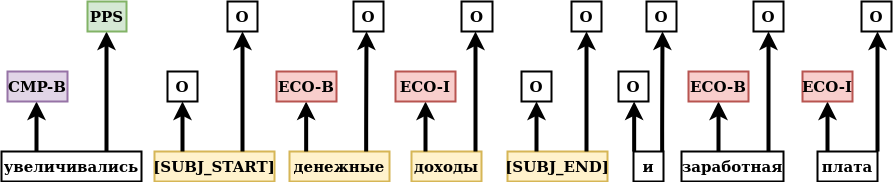
\includegraphics[scale=0.5]{pics/rel2}
		\caption{Joint relation extraction and named entity recognition training.}
		\label{fig:rel}
	\end{figure}
	
	
	For end-to-end relation extraction we went with a two-stage approach. At first we used the model from the first track to label named entities. After that using the provided named entity predictions we trained our model to infer semantic relations.
	
	In this task we used the same multilingual uncased BERT model as in subtask 1. However, to get simultaneous relation and named entity predictions on top of the model we added another dropout layer followed by tag and relation linear layers. We use weighted sum of cross entropy losses for tag and relation labeling as our final loss for optimization. Padding tokens do not contribute to our loss calculation.
	
	However, joint task learning only worsened our results and the best result at the validation set was
	
	\begin{table}[t!]
		\centering
		\scriptsize
		\begin{tabular}{lcc}%{llllllll}

			Method & test & dev \\

			test\_tag\_0.1\_and\_relation\_run\_predictions & 0.262 & 0.757 \\
			test\_tag\_0\_and\_relation\_run\_predictions & 0.249 & 0.784 \\

			$\star$ whole\_train\_tag\_0\_xlm\_r\_run\_predictions & {\bf 0.391} & 0.729 \\

			test\_xlm\_r\_tag\_0.1\_relation\_run\_predictions & 0.378 & 0.667 \\
			test\_xlm\_r\_tag\_0.1\_wd\_0.2\_relation\_run\_predictions & 0.356 & 0.668 \\
			test\_xlm\_r\_tag\_0.1\_relation\_drop\_0.2\_run\_predictions & 0.354 & 0.668 \\

			test\_xlm\_r\_tag\_0.01\_relation\_run\_predictions & 0.38 & 0.677 \\
			test\_xlm\_r\_tag\_relation\_run\_predictions & 0.27 & 0.679 \\
			test\_xlm\_r\_tag\_0\_relation\_run\_predictions & {\bf 0.389} & 0.678 \\
			test\_xlm\_r\_tag\_0.05\_relation\_run\_predictions & 0.389 & 0.685 \\
			test\_xlm\_r\_tag\_0.2\_relation\_run\_predictions & 0.339 & 0.662 \\ 
		\end{tabular}
		\caption{Subtask 2: Results on test and dev sets. $\star$ denotes out of competition result}
		\label{table:test_results_2}
	\end{table}
	
	The system showed 0.132 micro F1-score using public test data and it would have taken the first place among the provided systems, if we had managed to submit our solution before the deadline.
	\subsection{Subtask 2: Relation Extraction for given Named Entities}
	The model for this track is equivalent to the system used for end-to-end relation extraction. This track was very similar to end-to-end relation extraction. However, instead of using named entity labels predicted by our model, we could use the manual annotation provided by the organizers of the competition.
	
	We also attempted at using the multi-task learning procedure described in previous section. However, as in the previous case the quality deteriorated when the model was trained to predict named entity tags. Thus, the loss coefficient for named entity recognition was also set to zero.
	
	For subtask 2 we also tried a base XLM-RoBERTa \cite{roberta} model also provided by Hugging Face. RoBERTa is BERT inspired model which optimized many hyper-parameter choices in the underlying model. RoBERTa authors have replaced static masking with random masking during language training. They also removed additional sentence prediction loss, increased the batch size, trained on longer sequences and enhanced the original Wikipedia dataset with various Common Crawl datasets. All these adjustments helped RoBERTa to outperform BERT in many benchmarks such as GLUE or SQuAD 2.0.

	\section{Results}
	All in all, our named entity recognition model with micro F1-score equal to 0.561 took the first place in the competition. However, the results are lower than for other named entity recognition datasets (e.g. for the Ontonotes dataset Transformer-based models usually get > 0.85 in F1-score \footnote{see http://docs.deeppavlov.ai/en/master/features/models/ner.html}). It can be attributed to the small number of training examples and complexity of the domain.
	
	Our end-to-end relation extraction model despite being one of the best solutions at the competition was much worse than the model trained with manual annotations provided by the organizers. In future we will try to use approaches similar to pseudo labelling where we include only those named entity predictions that have high logit scores instead of all predictions. The difference in results also demonstrates that correct named entity labels are vital for relation extraction.
	
	Multi-task learning did not improve our results for this task as well. 
	\section{Conclusion}
	In this work we present our system for RuREBus challenge held together with Dialog 2020 conference. The task consisted of 3 tracks: named entity recognition, relation extraction with provided named entity tags and end-to-end relation extraction. All tracks we considered as sequence labelling problems. We show that sequence labelling might be a decent approach for the relation extraction problem. We also attempted to use joint-task learning. However, it did not improve our results on the validation dataset. The system took the first place in the named entity recognition track and the second place in the third track. For the second task we failed to submit the solution till the deadline but it was among the best systems. The systems for all tasks are based on Transformer models.
	
	\section{Acknowledgments}
	We would like to thank the organizers of the competition. We believe that their work will be very helpful for the development of natural language processing for the Russian language.
	\bibliography{dialogue}
	
	
\end{document}
